\SourcePage{694}{699}
\section{The low-energy theorem for bremsstrahlung}

In~\S~98 we examined photon emission during a collision of particles in the limit where the photon frequency tends to zero. The amplitude of that process was found to be inversely proportional to~$\omega$ and to have a simple expression in terms of the amplitude for the same collision without emission of the soft photon (we shall again refer to the latter, by convention, as the ``elastic'' scattering amplitude and denote it by~$M_{fi}^{(\mathrm{el})}$). At the next order in~$\omega$ we have
\begin{equation}
M_{fi}=M_{fi}^{(-1)}+M_{fi}^{(0)},
\tag{140.1}
\end{equation}
where the leading term~($\propto\omega^{-1}$) is supplemented by a correction independent of~$\omega$ ($\propto\omega^0$). We shall show that this correction, like the leading term, can be expressed through~$M_{fi}^{(\mathrm{el})}$ without reference to the details of the hadron's electromagnetic structure. This statement is called the \emph{low-energy theorem} for bremsstrahlung (\emph{F.~E. Low}, 1958).

We saw in~\S~98 that the main contribution to the amplitude for emission of a soft photon (the contribution corresponding to the first term in~(140.1)) comes from diagrams in which the initial or final particle emits the photon directly. These diagrams have the form
\begin{equation}
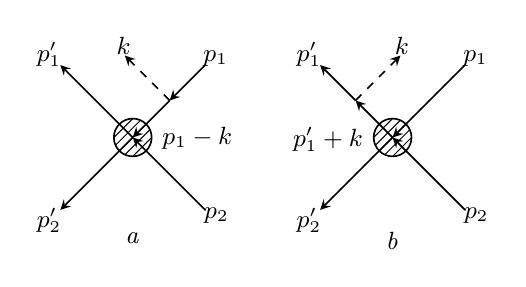
\begin{tikzpicture}[baseline=-.45ex,x=1cm,y=1cm,>=stealth,line width=.6pt,font=\small]
  \begin{scope}[xshift=-1.65cm]
    \coordinate (c) at (0,0);
    \coordinate (v) at (.47,.47);
    \draw[->] (c)--(-.92,.92);
    \draw[->] (c)--(-.92,-.92);
    \draw[->] (.92,-.92)--(c);
    \draw[->] (.92,.92)--(v);
    \draw[->] (v)--(c);
    \draw[dashed,->] (v)--(-.10,1.04);
    \begin{scope}
      \clip (c) circle (.24);
      \foreach \d in {-0.60,-0.48,...,0.60} {
        \draw[line width=.35pt] (-.55,\d-.55)--(.55,\d+.55);
      }
    \end{scope}
    \draw[fill=white,fill opacity=0] (c) circle (.24);
    \node[above left] at (-.78,.77) {$p'_1$};
    \node[above right] at (.77,.77) {$p_1$};
    \node[below left] at (-.78,-.77) {$p'_2$};
    \node[below right] at (.78,-.77) {$p_2$};
    \node[below right] at (.25,.26) {$p_1-k$};
    \node[above left] at (.10,.93) {$k$};
    \node[below] at (0,-1.08) {\textit{a}};
  \end{scope}
  \begin{scope}[xshift=1.65cm]
    \coordinate (c) at (0,0);
    \coordinate (v) at (-.47,.47);
    \draw[->] (.92,.92)--(c);
    \draw[->] (c)--(-.92,-.92);
    \draw[->] (.92,-.92)--(c);
    \draw[->] (c)--(v);
    \draw[->] (v)--(-.92,.92);
    \draw[dashed,->] (v)--(.10,1.04);
    \begin{scope}
      \clip (c) circle (.24);
      \foreach \d in {-0.60,-0.48,...,0.60} {
        \draw[line width=.35pt] (-.55,\d-.55)--(.55,\d+.55);
      }
    \end{scope}
    \draw[fill=white,fill opacity=0] (c) circle (.24);
    \node[above left] at (-.78,.77) {$p'_1$};
    \node[above right] at (.77,.77) {$p_1$};
    \node[below left] at (-.78,-.77) {$p'_2$};
    \node[below right] at (.78,-.77) {$p_2$};
    \node[below left] at (-.25,.26) {$p'_1+k$};
    \node[above right] at (-.10,.93) {$k$};
    \node[below] at (0,-1.08) {\textit{b}};
  \end{scope}
\end{tikzpicture}
\tag{140.2}
\end{equation}

\SourcePage{695}{700}
in contrast to diagrams of the form
\begin{equation}
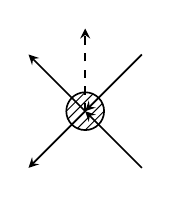
\begin{tikzpicture}[baseline=-.45ex,x=1cm,y=1cm,>=stealth,line width=.6pt]
  \coordinate (c) at (0,0);
  \draw[->] (c)--(-.72,.72);
  \draw[->] (c)--(-.72,-.72);
  \draw[->] (.72,.72)--(c);
  \draw[->] (.72,-.72)--(c);
  \draw[dashed,->] (c)--(0,1.05);
  \begin{scope}
    \clip (c) circle (.24);
    \foreach \d in {-0.60,-0.48,...,0.60} {
      \draw[line width=.35pt] (-.55,\d-.55)--(.55,\d+.55);
    }
  \end{scope}
  \draw[fill=white,fill opacity=0] (c) circle (.24);
\end{tikzpicture}
\tag{140.3}
\end{equation}
in which the photon line emerges from an internal part of the diagram. A graph of type~(140.2) can be divided into two pieces by cutting a single virtual-hadron line (that of the initial or the final hadron). In other words, such graphs display the property essential here: a one-particle intermediate state containing one hadron. As we saw in~\S~79, the unitarity requirement makes this property alone sufficient to produce a pole singularity in the amplitude.

For simplicity, suppose that only one of the two colliding hadrons (the first) carries electric charge and can therefore radiate, and that both hadrons have zero spin. The wave amplitudes~$u$ of these hadrons are scalars, which we set equal to~1.

The contribution from the pole part of diagram~(140.2,\textit{a}) is then
\begin{equation}
iM_{fi}^{(a)}=\sqrt{4\pi}\,e^*_{\mu}(2p_1^\mu-k^\mu)eF
\frac{1}{(p_1-k)^2-M^2}\,i\Gamma.
\tag{140.4}
\end{equation}
The first factor belongs to the photon~$k$ ($e_\mu$ is its polarization 4-vector). The second represents the electromagnetic hadron vertex (the solid dot in the diagram); it is written in the form~(138.5), with~$F$ the hadron form factor. The third factor is the propagator of the virtual hadron with momentum~$p_1-k$ (and mass~$M$). Finally, the factor~$i\Gamma$ denotes the entire remaining block. This block differs from the elastic-process amplitude
\begin{equation}
iM_{fi}^{(\mathrm{el})}
=
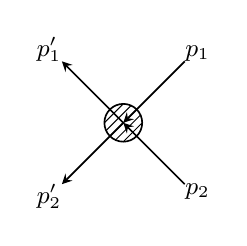
\begin{tikzpicture}[baseline=-.45ex,x=1cm,y=1cm,>=stealth,line width=.6pt,font=\small]
  \coordinate (c) at (0,0);
  \draw[->] (c)--(-.78,.78);
  \draw[->] (c)--(-.78,-.78);
  \draw[->] (.78,.78)--(c);
  \draw[->] (.78,-.78)--(c);
  \begin{scope}
    \clip (c) circle (.24);
    \foreach \d in {-0.60,-0.48,...,0.60} {
      \draw[line width=.35pt] (-.55,\d-.55)--(.55,\d+.55);
    }
  \end{scope}
  \draw[fill=white,fill opacity=0] (c) circle (.24);
  \node[above left] at (-.66,.65) {$p'_1$};
  \node[above right] at (.66,.65) {$p_1$};
  \node[below left] at (-.66,-.65) {$p'_2$};
  \node[below right] at (.66,-.65) {$p_2$};
\end{tikzpicture}
\tag{140.5}
\end{equation}
by having the real hadron~$p_1$ replaced with the virtual hadron~$p_1-k$.

The first terms in the expansion of~(140.4) in powers of~$k$ include: 1)~terms inversely proportional to~$\omega$; 2)~terms independent of~$\omega$ but dependent on the direction of~$\mathbf k$; and 3)~terms independent of~$\omega$ and also wholly independent of~$\mathbf k$. Terms of the third kind (and only that kind) are also contributed by the ``nonsingular'' diagrams of type~(140.3),

\SourcePage{696}{701}
which contain no pole singularity, and by the non-pole parts of diagrams~(140.2). We shall see that gauge invariance fixes all such terms together uniquely from those of the first two types, so no separate calculation of them is required.

The amplitude of the elastic process~(140.5) depends on only two invariant variables:
\begin{equation}
s=(p_1+p_2)^2=(p'_1+p'_2)^2,\qquad t=(p'_2-p_2)^2.
\tag{140.6}
\end{equation}
Replacing $p_1$ by $p_1-k$ not only changes~$s$ to~$(p_1-k+p_2)^2$, but also introduces dependence on the new variable
\[
(p_1-k)^2-M^2=-2(p_1k),
\]
which characterizes the ``unphysicality'' of the momentum~$p_1-k$. The first term alone in the expansion in this new (small) variable, however, removes the singularity in the amplitude~(140.4); it can consequently contribute only terms independent of~$k$, which, as explained above, are not yet of interest to us. We therefore reach the important conclusion that~$\Gamma$ in~(140.4) may be replaced by the physical amplitude~$M_{fi}^{(\mathrm{el})}(s,t)$, provided that within this amplitude we make the replacement
\begin{equation}
s\to(p_1+p_2-k)^2=s-2k(p_1+p_2).
\tag{140.7}
\end{equation}
The first terms of its expansion are
\[
\Gamma\to M_{fi}^{(\mathrm{el})}(s,t)
-2(kp_1+kp_2)\left(\frac{\partial M_{fi}^{(\mathrm{el})}}{\partial s}\right)_t.
\]

For the same reason, it is immaterial that the electromagnetic form factor~$F$ here belongs to a vertex for which only one of its two hadron legs ($p_1$ and~$p_1-k$) is physical. It may therefore be replaced by the form factor considered in~\S~138 for a vertex with two physical legs. Since the photon~$k$ is real in the present case, $F(k^2)=F(0)=Z_1$, where $eZ_1$ is the hadron charge.

Thus, from~(140.8) we find
\begin{equation}
\begin{aligned}
M_{fi}^{a}={}&Z_1e\sqrt{4\pi}\,
\frac{2(e^*p_1)}{-2(kp_1)}M_{fi}^{(\mathrm{el})}-{}\\
&{}-Z_1e\sqrt{4\pi}\,2(e^*p_1)\frac{1}{-2(kp_1)}
\cdot2(p_2k)\frac{\partial M_{fi}^{(\mathrm{el})}}{\partial s}+\ldots,
\end{aligned}
\tag{140.8}
\end{equation}
where the ellipsis denotes terms wholly independent of~$k$ (whereas the second term in~(140.8) depends on the direction of~$\mathbf k$). In the same way, the contribution to~$M_{fi}$ from diagram~(140.2,\textit{b})

\SourcePage{697}{702}
is obtained from~(140.8) by replacing $p_1$, $p_2$, and~$k$ with $p'_1$, $p'_2$, and~$-k$. The leading term in the expansion then gives the expression already found earlier:
\begin{equation}
M_{fi}^{(-1)}=Z_1e\sqrt{4\pi}
\left(\frac{(p'_1e^*)}{(p'_1k)}-\frac{(p_1e^*)}{(p_1k)}\right)
M_{fi}^{(\mathrm{el})}
\tag{140.9}
\end{equation}
(cf.~(98.5)).

The terms independent of~$k$ can instead be determined by requiring gauge invariance of the complete amplitude. More precisely, it must be unchanged under $e^*\to e^*+\mathop{\rm const}\nolimits\cdot k$; that is, it must have the form $M_{fi}=e^*_{\mu}J^\mu$, with $k_\mu J^\mu=0$. It is readily seen that this requires adding to~(140.8) the $k$-independent term
\[
-2Z_1e\sqrt{4\pi}\,(p_2e^*),
\]
and likewise for diagram~(140.2,\textit{b}). The final result is therefore
\begin{equation}
M_{fi}^{(0)}=2Z_1e\sqrt{4\pi}\,e^*_{\mu}
\left[p_1^\mu\frac{(p_2k)}{(p_1k)}-p_2^\mu
+p_1'{}^\mu\frac{(p'_2k)}{(p'_1k)}-p_2'{}^\mu\right]
\frac{\partial M_{fi}^{(\mathrm{el})}}{\partial s}.
\tag{140.10}
\end{equation}
This formula supplies the required result. It can be put in a more compact form by making the identity substitution
\[
2p_{2\nu}\left(\frac{\partial}{\partial s}\right)_t
=\left(\frac{\partial}{\partial p_1^\nu}\right)_{p'_1,p_2,p'_2}
\]
(and similarly for~$\partial/\partial p_1'{}^\nu$), and by introducing the differential operators
\begin{equation}
\widehat d_{1\mu}=\frac{p_{1\mu}}{(p_1k)}k^\nu\frac{\partial}{\partial p_1^\nu}
-\frac{\partial}{\partial p_1^\mu}
\tag{140.11}
\end{equation}
(with~$\widehat d_{1'\mu}$ defined analogously). Then
\begin{equation}
M_{fi}^{(0)}=Z_1e\sqrt{4\pi}\,e^*_{\mu}
\bigl(\widehat d_1^\mu+\widehat d_{1'}^\mu\bigr)M_{fi}^{(\mathrm{el})}.
\tag{140.12}
\end{equation}
To the accuracy required, the cross section is determined by the squared amplitude
\begin{equation}
|M_{fi}|^2=|M_{fi}^{(-1)}|^2
+2\mathop{\rm Re}\nolimits\bigl(M_{fi}^{(-1)}M_{fi}^{(0)*}\bigr).
\tag{140.13}
\end{equation}
The second term gives the correction sought for the radiation cross section. On summing over the photon polarizations, this correction becomes
\begin{equation}
-4\pi(Z_1e)^2
\left(\frac{p'^\mu}{(p'k)}-\frac{p^\mu}{(pk)}\right)
(\widehat d_1+\widehat d_{1'})_\mu|M_{fi}^{(\mathrm{el})}|^2.
\tag{140.14}
\end{equation}

\SourcePage{698}{703}
Thus the correction to the radiation cross section is expressed through the elastic-process cross section and its derivative with respect to~$s$.

If the charged hadron has spin~$1/2$, the essential reasoning of the calculation remains unchanged. Only the particular forms of the vertices and propagators are different. After averaging over the hadron and photon polarizations, formula~(140.14) nevertheless remains valid (\emph{T.~N. Burnett, N.~M. Kroll}, 1968).
